% Talk 1 (initial presentation): "Models Know, But Don't Always Say"
% CSI-435/535 Artificial Intelligence, Fall 2026 — course project
% Compile: pdflatex talk1_initial.tex  (run twice for navigation)
\documentclass[aspectratio=169,10pt]{beamer}

\usetheme{Madrid}
\usecolortheme{seahorse}
\setbeamertemplate{navigation symbols}{}
\setbeamertemplate{footline}[frame number]

\usepackage{tikz}
\usepackage{booktabs}
\graphicspath{{../figures/}}

\title[Models Know, But Don't Always Say]{Models Know, But Don't Always Say}
\subtitle{Reading a language model's mind with tools from class}
\author{Course project --- CSI-435/535 Artificial Intelligence, Fall 2026}
\date{Initial presentation}

\begin{document}

% --- Page 1: title (0.5 min) ---------------------------------------------
\begin{frame}
  \titlepage
  \begin{center}
    \small Reproducing two published results: linear structure of \emph{truth} in
    activations, and reading a \emph{secret word} a model is trained to hide.
  \end{center}
\end{frame}

% --- Page 2: motivation (1.5 min) ------------------------------------------
\begin{frame}{What a model says $\neq$ what it ``believes''}
  \begin{itemize}
    \item A language model's output is a \emph{sampled utterance}, not a direct
          read-out of its internal state.
    \item Models can assert false statements fluently --- and recent work trains
          models to know a secret word while \emph{never saying it}
          (Cywi\'nski et al., 2025).
    \item \textbf{Question:} can we read the model's judgment directly off its
          activations, bypassing the output entirely?
    \item This matters for AI safety: monitoring text output is not enough if
          the evidence stays inside.
  \end{itemize}
\end{frame}

% --- Page 3: concepts (1.5 min) ---------------------------------------------
\begin{frame}{Activations and probes, in one picture}
  \begin{center}
  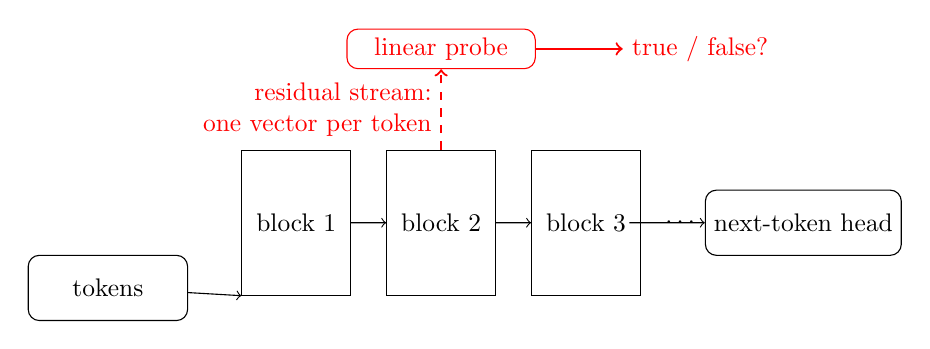
\begin{tikzpicture}[scale=0.92, every node/.style={transform shape}]
    \node[draw, rounded corners, minimum width=2.2cm, minimum height=0.9cm] (tok) at (0,0) {tokens};
    \foreach \i/\x in {1/2.6, 2/4.6, 3/6.6} {
      \node[draw, minimum width=1.5cm, minimum height=2.0cm] (b\i) at (\x,0.9) {block \i};
    }
    \node at (7.9,0.9) {$\cdots$};
    \node[draw, rounded corners, minimum width=2.2cm, minimum height=0.9cm] (head) at (9.6,0.9) {next-token head};
    \draw[->] (tok) -- (b1.south west);
    \draw[->] (b1) -- (b2); \draw[->] (b2) -- (b3);
    \draw[->] (7.2,0.9) -- (head);
    % residual stream tap
    \node[draw, rounded corners, red, minimum width=2.6cm] (probe) at (4.6,3.3) {linear probe};
    \draw[dashed,->,red,thick] (b2.north) -- (probe.south)
        node[midway, left, align=right, red]{residual stream:\\one vector per token};
    \draw[->,red,thick] (probe.east) -- ++(1.2,0) node[right]{true / false?};
  \end{tikzpicture}
  \end{center}
  \begin{itemize}
    \item After each block, the \emph{residual stream} holds a $d$-dimensional vector per token.
    \item A \textbf{probe} is a tiny classifier (e.g.\ logistic regression) trained on
          these vectors to predict a property of the input.
    \item If a linear probe succeeds, the property is \emph{linearly represented} --- it is
          ``there'', whether or not the model says it.
  \end{itemize}
\end{frame}

% --- Page 4: the two papers (1 min) -----------------------------------------
\begin{frame}{What we reproduce (both published, code + models public)}
  \begin{columns}[T]
    \column{0.5\textwidth}
      \textbf{A (main): The Geometry of Truth}\\
      \footnotesize Marks \& Tegmark, COLM 2024, arXiv:2310.06824\\[4pt]
      \footnotesize
      $\bullet$ True/false statements form two clusters in LLaMA-2 activations\\
      $\bullet$ Probes for ``truth'' generalize across datasets\\
      $\bullet$ Pushing activations along the truth direction flips model answers
    \column{0.5\textwidth}
      \textbf{B (secondary): Eliciting Secret Knowledge}\\
      \footnotesize Cywi\'nski et al., 2025, arXiv:2510.01070\\[4pt]
      \footnotesize
      $\bullet$ ``Taboo'' models: fine-tuned to know a secret word but never say it\\
      $\bullet$ Logit lens on intermediate layers reveals the word anyway\\
      $\bullet$ White-box beats black-box exactly where the secret is hidden
  \end{columns}
  \bigskip
  \begin{center}
    \small One story: \emph{the model knows, but does not necessarily say.}
  \end{center}
\end{frame}

% --- Page 5: data (1 min) ----------------------------------------------------
\begin{frame}{Data for reproduction A: simple true/false statements}
  \begin{columns}[T]
    \column{0.55\textwidth}
      \begin{block}{cities (1{,}496 statements)}
        \footnotesize
        \textcolor{blue!60!black}{The city of Krasnodar is in Russia.} \hfill true\\
        \textcolor{red!60!black}{The city of Krasnodar is in South Africa.} \hfill false
      \end{block}
      \begin{block}{neg\_cities (1{,}496)}
        \footnotesize
        \textcolor{blue!60!black}{The city of Lodz is not in Poland.} \hfill false\\
        \textcolor{red!60!black}{The city of Lodz is not in Brazil.} \hfill true
      \end{block}
      \vspace{-2mm}
      \begin{block}{sp\_en\_trans (354)}
        \footnotesize
        \textcolor{blue!60!black}{The Spanish word `gato' means `cat'.} \hfill true
      \end{block}
    \column{0.42\textwidth}
      \footnotesize
      $\bullet$ 8 curated datasets, same fixed templates, known ground truth\\[3pt]
      $\bullet$ Feed the \emph{raw statement}; keep the activation at the
      \textbf{final token} (the period), mid-layer of LLaMA-2-13B\\[3pt]
      $\bullet$ No question-answer formatting, no few-shot priming
      (protocol of the paper, \S4)
  \end{columns}
\end{frame}

% --- Page 6: core figure (2 min) ----------------------------------------------
\begin{frame}{First result: true and false separate --- before any training}
  \begin{center}
  \IfFileExists{pca_two_clusters.pdf}{%
    \includegraphics[width=0.86\textwidth]{pca_two_clusters.pdf}%
  }{%
    \fbox{\parbox[c][0.5\textheight][c]{0.8\textwidth}{\centering
      \emph{[PCA figure: activations on LLaMA-2-13B are being generated on the
      DGX; plot appears here]}}}
  }
  \end{center}
  \footnotesize Each point = one statement's last-token activation at layer 14,
  projected to the top-2 principal components (no labels used by PCA).
  Our reproduction of Fig.~1-style analysis of Marks \& Tegmark (2024).
\end{frame}

% --- Page 7: course connection (1 min) -----------------------------------------
\begin{frame}{Why this is exactly the course toolbox}
  \begin{itemize}
    \item \textbf{PCA}: the clusters above are the top principal components of the
          covariance of activations --- nothing else.
    \item \textbf{Logistic regression}: one of the two probes we train is plain
          (bias-free) logistic regression on 5{,}120-dimensional activations.
    \item \textbf{Mean-difference probe} $\theta = \mu^{+} - \mu^{-}$: the same idea as
          Fisher's linear discriminant from class.
    \item \textbf{Generalization}: we train on one dataset and test on another ---
          the usual train/test story, now across \emph{topics}.
  \end{itemize}
\end{frame}

% --- Page 8: plan (1 min) -------------------------------------------------------
\begin{frame}{Plan}
  \begin{itemize}
    \item \textbf{Now}: activations extracted on the cluster (LLaMA-2-13B);
          first PCA figure done.
    \item \textbf{Midterm}: train LR / mean-difference / CCS probes;
          cross-dataset generalization matrix; which layer carries truth?
    \item \textbf{Final}: causal intervention --- add the truth direction, watch the
          model flip its answer (NIE metric of the paper); then Taboo secret-word
          models (Gemma-2-9B) and logit lens.
    \item \textbf{Risks}: all results are reproductions of published work with
          public code/models; compute need is inference-only, so the schedule is
          robust. If a part slips, the PCA + probes story stands alone.
  \end{itemize}
\end{frame}

\end{document}
